\section{Size}

For the purposes of talking about size-change termination, we also need to
define the notion of size, and be sure to do so in such a way so that all
possible data values are well-founded.

\begin{definition}\label{definition:size}

Size of a value in \D{} is the number of nodes in the tree representing
that value.

\end{definition}

The ``well-foundedness'' of \D{}'s data values, given such a definition can be
argued for by proving a bijective relation between $\mathbb{B}$ and
$\mathbb{N}$. This would imply that we can define the relation $<$ on \D{}'s
data values, which we know to be well-founded.

We start by formally proving that \referToDefinition{size} yields a many-to-one
mapping of \D{}'s data values to the natural numbers.

First, we prove, by induction, that any natural number can be represented in
\D{}:

\begin{proof}\ \\

\begin{description}[\setleftmargin{70pt}\setlabelstyle{\bf}]

\item [Base] The atom $0$ has no nodes, and hence represents the value $0$.

\item [Assumption] If we can represent the $n\in\mathbb{N}$ in \D{}, then
we can also represent the number $n+1\in\mathbb{N}$. 

\item [Induction] Let $n$ be represented by some binary tree $A$, then $n+1$
can be represented by $0\cdot A$. 

\end{description}

\end{proof}

Second, we prove, also by induction, that any value in \D{} has one and only
one representation in $\mathbb{N}$.

\begin{proof}\ \\

\begin{description}[\setleftmargin{70pt}\setlabelstyle{\bf}]

\item [Base] The atom $0$ has no nodes, and hence corresponds only to the value
$0$.

\item [Assumption]

\begin{enumerate}

\item If the binary tree $A$ has only one representation $n\in\mathbb{N}$, then
$\left|0\cdot A\right|\equiv n+1$ and $\left|A\cdot 0\right|\equiv n+1$.

\item If the binary tree $A$ has only one representation $n\in\mathbb{N}$, and
the binary tree $B$ has only one representation $m\in\mathbb{N}$, then
$\left|A\cdot B\right|\equiv n+m+1$ and $\left|B\cdot A\right|\equiv n+m+1$.

\end{enumerate}

\item [Induction]

By definition of the binary function $\cdot$, any given node $A$ with left
child $A_{left}$ and right child $A_{right}$ has the size:

$$\left|A\right|=1+\left|A_{left}\right|+\left|A_{right}\right|$$

Hence, any value in \D{} must have one and only one representation in
$\mathbb{N}$.

\end{description}

\end{proof}

\referToDefinition{size} \emph{almost} allows us to devise an algorithm to
compare the sizes of data values. The problem withstanding is that two
different values can have rather diverging tree representations. Hence,
comparing them, using only the operations defined in \referToSection{d-sos}, is
seemingly impossible unless we initially, or along the way, transform the
binary trees being compared into some sort of a \emph{standard representation}.
We'll define this representation, recursively, as follows:

\begin{definition}\label{definition:standard-representation}

A binary tree in standard representation is a binary tree that either is a leaf
or a node having a leaf as it's left child and a binary tree in standard
representation as it's right child.

\end{definition}

Intuitively, a binary tree in standard representation is just a tree that only
descends along the right side. Comparing the sizes of two trees in this
representation is just a matter of walking the descending in the two trees
simultaneously, until one of them, or both, bottom out. If there is a tree that
bottoms out strictly before another, that is the lesser tree by
\referToDefinition{size}. \referToFigure{standard-representation} showcases
some examples.

\begin{figure}[htbp!]
\centering
\subfigure[{Not in standard representation}]
{
  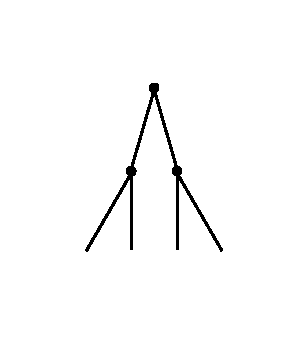
\includegraphics[scale=1]{figures/first-non-standard}
}
\subfigure[{Not in standard representation}]
{
  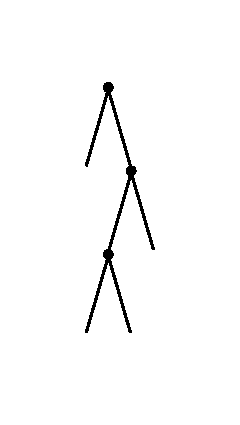
\includegraphics[scale=1]{figures/second-non-standard}
}
\subfigure[{Standard representation}]
{
  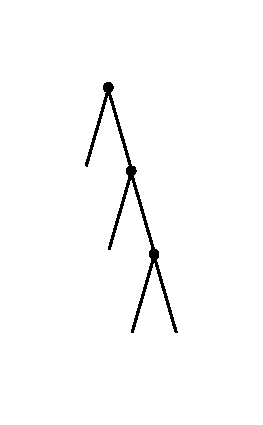
\includegraphics[scale=1]{figures/standard}
}
\caption[]{Three trees of various shapes but equal size.}
\label{figure:standard-representation}
\end{figure}

\subsection{\mono{normalize/1}}

\begin{verbatim}
normalize a = normalize-aux a 0 0

normalize-aux 0     0     an = an
normalize-aux 0     bl.br an = normalize-aux bl br    an
normalize-aux 0.ar  b     an = normalize-aux ar b     0.an
normalize-aux al.0  b     an = normalize-aux al b     0.an
normalize-aux al.ar b     an = normalize-aux ar al.b  0.an

\end{verbatim}

\subsubsection{Correctness}

\mono{normalize/1} makes use of an auxiliary procedure, \mono{normalize-aux/3},
for which we can provide the following argument descriptions:

\begin{enumerate}

\item The tree to be normalized.

\item An auxiliary tree.

\item A normalized tree.

\end{enumerate} 

The idea of the algorithm is to move right-wise down the tree to be normalized,
constructing an auxiliary tree containing all left-wise child nodes, if any.

The return value is the normalized tree, i.e. the third argument. Hence, we
must increase the size of the normalized tree each time we move right-wise down
the tree to be normalized.

Once we reach the right-most leaf of the tree to be normalized we return the
normalized tree if the auxiliary tree is empty. Otherwise, we normalize the
right child of the auxilary tree, with the left child of the auxiliary as the
new auxiliary tree, and the normalized tree constructed thus far as the initial
normalized tree.

\subsubsection{Time complexity}

Coming soon..

\subsubsection{Space complexity}

Coming soon..

\subsection{\mono{less/2}}\label{section:d-size-less}

We'll define the function \mono{normalize/1} further below to transform any
\D{} value into it's standard representation. For now we'll assume that we have
such a function in scope and define \mono{less/2} for determining whether the
value of the first argument is strictly less than the value of the second
argument.

In order to define such a boolean-valued function we need a convention for
representing the boolean values $true$ and $false$ in \D{}. We'll adopt the
C-like convention:

\begin{definition}

A $false$ value is represented by a leaf tree. A $true$ value is represented by
a non-leaf tree, i.e. a node.

\end{definition}

We're now ready to define the function \mono{less/2}:

\begin{lstlisting}[label={listing:d-less},caption={A definition of the \mono{less/2} function.}]
less a b := normalized-less (normalize a) (normalize b)

normalized-less 0 b := b
normalized-less _ 0 := 0
normalized-less _.a _.b := normalized-less a b
\end{lstlisting}

\subsubsection{Correctness}

\begin{proof}

Given \referToDefinition{standard-representation}, and the assumption that
$\proc{Normalize}(A)$ computes the standard representation of $A$, we know the
following:

\begin{enumerate}

\item $\left|A\right|\equiv\left|\proc{Normalize}(A)\right|$.

\item We'll walk through all the nodes if we perform a recursive
right-child-walk starting at $A$.

\item The same holds for $B$.

\end{enumerate}

It is also easy to see from lines
\ref{normalized-less-init-start}:\ref{normalized-less-init-end} that
$\proc{NormalizedLess}$ stops as soon as we reach the ``bottom'' of either $A$
or $B$.

Given \referToDefinition{size}, $A<B$ iff it bottoms out before $B$, that is,
we reach an instance of the recursion where both $IsLeaf(A)$ and $IsNode(B)$
hold.  In all other cases $A\geq B$, the cases specifically are:

\begin{itemize}

\item $IsLeaf(A)$ and $IsLeaf(B)$, then $\left|A\right|\equiv \left|B\right|$.

\item $IsNode(A)$ and $IsLeaf(B)$, then $\left|A\right|>\left|B\right|$

\end{itemize}

Last but not least, due to all data values being finite, eventually one of the
trees does bottom out.

\end{proof}

\subsubsection{Time complexity}

Given that the binary trees $A$ and $B$ are in standard representation when we
enter the auxiliary procedure, $\proc{NormalizedLess}$, it is fairly easy to
get an upper bound on the running time of $\proc{NormalizedLess}$ itself.

Indeed, the running time of $\proc{NormalizedLess}$ itself is
$O\left(\proc{Max}\left(\left|A\right|,\left|B\right|\right)\right)$, since we
just walk down the trees until one of them bottoms out. 

We haven't yet defined the procedure $\proc{Normalize}$ yet. Hence, the only
thing that we can say about the running time of $\proc{Less}$ in general is
that it is $O\left(\proc{Normalize}(A) + \proc{Normalize}(B) +
\proc{Max}\left(\left|A\right|,\left|B\right|\right) \right)$.

\subsubsection{Space complexity}

Coming soon..
